%% ============================================================
%%  CoG2026_NPC_Dialogue.tex
%%  COMPILE WITH:  pdflatex CoG2026_NPC_Dialogue.tex
%%  (NOT XeLaTeX -- IEEEtran conference requires pdflatex)
%% ============================================================
\documentclass[conference]{IEEEtran}
\IEEEoverridecommandlockouts
%% ---- Packages ----
\usepackage{cite}
\usepackage{amsmath,amssymb,amsfonts}
\usepackage{mathtools}
\usepackage{graphicx}
\usepackage{textcomp}
\usepackage{xcolor}
\usepackage{booktabs}
\usepackage{array}
\usepackage{multirow}
\usepackage{url}
\usepackage{tikz}
\usetikzlibrary{arrows.meta,positioning}

\def\BibTeX{{\rm B\kern-.05em{\sc i\kern-.025em b}\kern-.08em
    T\kern-.1667em\lower.7ex\hbox{E}\kern-.125emX}}

%% ============================================================
%%  DOUBLE-ANONYMOUS SUBMISSION -- CoG 2026
%%  Author names and affiliations omitted per review policy.
%%  Camera-ready version will restore full author information.
%% ============================================================
\title{Dynamic Game-State-Informed Fine-Tuned Language Models\\
for Context-Aware NPC Dialogue in Narrative Games}

\author{\IEEEauthorblockN{Anonymous Author(s)}
\IEEEauthorblockA{Affiliation omitted for double-anonymous review}}

\begin{document}
\maketitle

%% ============================================================
\begin{abstract}
Deploying large language models for real-time NPC dialogue in
narrative games introduces three interrelated challenges:
\emph{context drift} as game state evolves across play sessions,
\emph{adversarial retrieval vulnerabilities} that can override
character-role policies, and a persistent \emph{harness-to-runtime
gap} between offline benchmark results and live engine behavior.
We address all three through an end-to-end Unreal Engine~5
dialogue pipeline coupling bounded game-state serialization,
guarded hybrid retrieval with adversarial-risk penalties, a
locally fine-tuned model (Phi-3 Mini, 3.8B parameters; QLoRA~SFT
followed by DPO), and post-generation response control with
verified Python/C++ behavioral parity. A conjunctive evidence
gate~$\Gamma$ requires convergent support across five evaluation
axes before any experimental conclusion is accepted. On a
112-scenario fixed-arm benchmark, controlled contextual inference
yields statistically significant improvements over raw-context
generation across all four core quality dimensions---context
relevance~($+0.184$), persona consistency~($+0.151$),
naturalness~($+0.097$), and overall quality~($+0.144$)---with all
bootstrap confidence intervals strictly above zero. Guarded
retrieval eliminates adversarial instruction compliance in both
tested attack families (attack success rate reduced from
$1.0$~to~$0.0$). These quality gains incur a measurable latency
overhead ($+463$\,ms), which we report as an explicit deployment
trade-off. A further structural finding is that retrieval quality
and response admissibility constitute separable control problems,
implying that modular, independently calibrated guard and control
stages are preferable to monolithic post-processing for NPC
dialogue systems.
\end{abstract}

\begin{IEEEkeywords}
NPC dialogue, game AI, local LLM, UE5, QLoRA, DPO,
game-state conditioning, guarded retrieval, adversarial
robustness, conjunctive evidence gate, fixed-arm benchmark,
response control, behavioral parity
\end{IEEEkeywords}

%% ============================================================
\section{Introduction}

Narrative games demand NPC dialogue that is fluent, in-character,
and continuously responsive to an evolving game world. Hand-crafted
dialogue trees remain the production standard, but their authoring
cost scales poorly as narrative scope expands
\cite{Gallotta2024Survey,Sweetser2024Scoping}. LLM-driven
generation offers open-ended flexibility, yet introduces
failure modes that are largely unaddressed in prior work:
\textit{context drift} over multi-turn play
\cite{Park2023GenerativeAgents}, \textit{adversarial compliance}
when retrieved passages are poisoned or authority-spoofed, and
a \textit{harness-to-runtime gap} in which benchmark results do
not transfer to live engine behavior.

Prior work demonstrates user-experience gains with LLM-driven NPCs
\cite{Rao2024Minecraft,Christiansen2024Presence,Wevelsiep2025Voice},
but system-level evidence remains thin: scenario coverage is
typically narrow, adversarial stress-testing is largely absent,
and evaluation harnesses are rarely verified against deployed
engine code \cite{Gallotta2024Survey}. These gaps matter
practically---a system that performs well offline may still fail
in the engine loop if context extraction, retrieval ranking, and
post-generation control are loosely coupled.

This paper closes all three gaps through an end-to-end UE5
dialogue pipeline in which every architectural component is
paired with a pre-registered evaluation criterion. Our
contributions are:

\begin{itemize}
\item A \textbf{six-stage runtime architecture} integrating
Blackboard-based game-state serialization, structured prompt
compilation, guarded hybrid retrieval, locally fine-tuned
generation, and post-generation response control with
\textit{verified} Python/C++ behavioral parity---eliminating
the harness-to-runtime gap by construction.
\item A \textbf{two-stage domain adaptation pipeline}
(QLoRA SFT $\to$ DPO) on Phi-3 Mini Instruct (3.8B) enabling
single-GPU deployment, augmented by a pairwise reranker trained
on hard-negative adversarial passage pairs
(pairwise accuracy $0.956$, 95\% CI $[0.937,\,0.974]$).
\item A \textbf{conjunctive evidence gate} $\Gamma$ requiring
convergent support across five axes---scenario coverage,
statistical significance, human evaluation, retrieval quality,
and adversarial security---before any conclusion is confirmed.
Of 23 recorded benchmark runs, only 5 satisfied $\Gamma{=}1$,
illustrating that partial-evidence acceptance is a real risk
in iterative game AI development.
\item A \textbf{separability finding}: ablation with the response
controller removed shows that retrieval quality and response
admissibility are independent control problems---context omission
and persona drift increase even when retrieval quality is held
constant, confirming that they cannot be collapsed into a single
post-processing stage.
\item A \textbf{112-scenario fixed-arm benchmark} with paired
bootstrap inference ($B{=}5{,}000$), blind human evaluation
($\kappa{=}0.533$, three raters, 324 judgments), adversarial
stress-testing across two attack families, and UE5 operational
metrics---explicitly reporting both quality gains and latency
costs.
\end{itemize}

\noindent The evaluation addresses four research questions.
\textbf{RQ1}: Does controlled contextual inference yield
measurable quality improvements over raw-context generation
under identical scenario and decoding conditions?
\textbf{RQ2}: Does the controlled system maintain a cross-condition
quality advantage over uncontextualized external baselines?
\textbf{RQ3}: Does guarded retrieval significantly reduce
adversarial instruction compliance under evidence poisoning
and trust-spoofing attacks?
\textbf{RQ4}: What quality--latency trade-offs arise when
guard and response-control mechanisms are simultaneously
activated?

%% ============================================================
\section{Related Work}

\subsection{LLMs as NPC and Game Agents}
Generative Agents \cite{Park2023GenerativeAgents} showed
reflective memory loops produce emergent social behavior in
sandbox simulations. Voyager \cite{Wang2024Voyager} demonstrated
open-ended task mastery in Minecraft via skill-library curriculum
generation. SIMA \cite{DeepMind2024SIMA} generalized
instruction-following across diverse 3D environments.
Voice-controlled NPC systems \cite{Wevelsiep2025Voice} and
LLM-driven quest collaboration \cite{Rao2024Minecraft} improve
player presence and engagement. These systems advance broad
behavioral capability but treat response admissibility and
engine-level runtime stability as secondary concerns. Persona
consistency under role-policy constraints and the behavioral gap
between an evaluation harness and a live engine remain largely
uncharacterized---the precise gap this work addresses.

\subsection{Retrieval-Augmented Generation and Adversarial Risks}
RAG \cite{Lewis2020RAG} grounds generation in retrieved evidence;
dense passage retrieval \cite{Karpukhin2020DPR} and efficient
similarity indexing \cite{Johnson2021FAISS} underpin the dense
branch. Self-RAG \cite{Asai2024SelfRAG} improves quality through
adaptive self-critique, and graph-based variants
\cite{Edge2024GraphRAG} extend the paradigm. However, standard
retrieval assumes a benign corpus. Indirect prompt injection
\cite{Greshake2023PromptInjection} subverts application behavior
through retrieved context; knowledge poisoning
\cite{Zou2025PoisonedRAG} steers outputs with a small number of
injected passages; and adversarial instructional prompts
\cite{Chaturvedi2025AIP} can hijack retrieval even when user
queries are clean. For NPC systems these risks are acute:
successful poisoning directly causes role-policy violations
visible to the player.

\subsection{Efficient Model Adaptation}
LoRA and QLoRA \cite{Hu2021LoRA,Dettmers2023QLoRA} enable
domain fine-tuning within single-GPU memory budgets. Instruction
tuning \cite{Wei2022Flan} and RLHF \cite{Ouyang2022InstructGPT}
shape model behavior; DPO \cite{Rafailov2023DPO} achieves
preference alignment without a separate reward model. We apply
these techniques sequentially on a domain-specific NPC corpus.

\subsection{Evaluation Methodology for Dialogue Systems}
Standard overlap-based metrics are insufficient for interactive
dialogue \cite{Yeh2021DialogMetrics}. LLM-as-judge frameworks
\cite{Liu2023GEval,Zheng2023MTBench} introduce position and
length biases \cite{Gu2026LLMJudge}. Our framework addresses
this by combining automated metrics, paired bootstrap inference,
blind human evaluation, and adversarial testing under a
conjunctive evidence gate---requiring all axes to pass before
a conclusion is confirmed.

\subsection{System Positioning}

Table~\ref{tab:position} contrasts representative prior systems
across the five dimensions that define the scope of this work.
No existing system addresses all five simultaneously within a
live game engine runtime.

\begin{table}[!t]
\renewcommand{\arraystretch}{1.15}
\caption{Positioning of representative systems across key
evaluation dimensions. $\bullet$=addressed;
$\circ$=partially addressed; ---=not addressed.}
\label{tab:position}
\centering
\setlength{\tabcolsep}{2.5pt}
\begin{tabular}{lccccc}
\toprule
System & \rotatebox{70}{State Ground.} & \rotatebox{70}{Adv. Guard} &
\rotatebox{70}{Runtime Par.} & \rotatebox{70}{Stat. Evid.} &
\rotatebox{70}{Adv. Eval.} \\
\midrule
Gen. Agents \cite{Park2023GenerativeAgents} & $\circ$ & --- & --- & --- & --- \\
Voyager \cite{Wang2024Voyager}       & --- & --- & $\circ$ & --- & --- \\
Minecraft NPC \cite{Rao2024Minecraft}& $\circ$ & --- & $\circ$ & $\circ$ & --- \\
Self-RAG \cite{Asai2024SelfRAG}      & --- & $\circ$ & --- & $\circ$ & --- \\
\textbf{This work}                   & $\bullet$ & $\bullet$ & $\bullet$ & $\bullet$ & $\bullet$ \\
\bottomrule
\end{tabular}
\end{table}

%% ============================================================
\section{System Architecture}
\label{sec:arch}

\subsection{Runtime Pipeline Overview}

Fig.~\ref{fig:arch} illustrates the six-stage online pipeline.
At each turn: the UE5 AI controller emits a bounded game-state
snapshot (\textbf{S1}); a context extractor normalizes it into
key-value fields (\textbf{S2}); a prompt compiler assembles the
persona, dynamic context, and retrieved evidence within a fixed
token budget (\textbf{S3}); the guarded retriever ranks passages
by relevance and adversarial risk (\textbf{S4}); the local LLM
generates a candidate response (\textbf{S5}); the response
controller evaluates admissibility and applies fallback if
needed (\textbf{S6}); and the accepted response is committed to
memory.

\begin{figure}[!t]
\centering
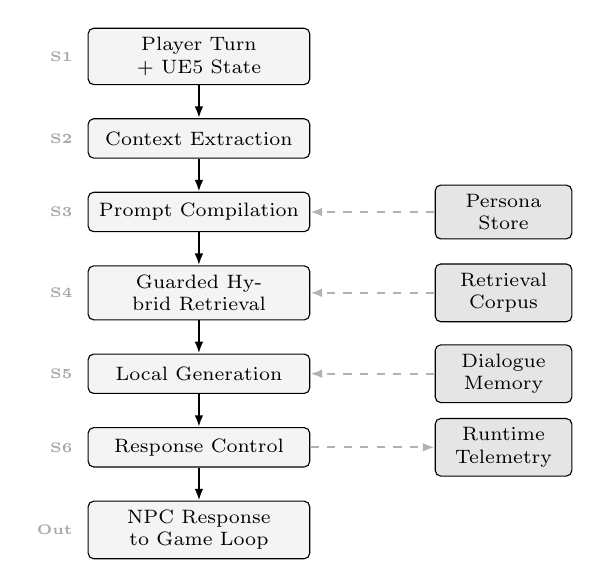
\begin{tikzpicture}[
  font=\scriptsize,
  node distance=0.42cm and 1.58cm,
  box/.style   = {draw, rounded corners=2pt, minimum height=0.50cm,
                  text width=2.58cm, align=center, fill=gray!9},
  store/.style = {draw, rounded corners=2pt, minimum height=0.44cm,
                  text width=1.50cm, align=center, fill=gray!20},
  arr/.style   = {-{Latex[length=1.5mm,width=1.1mm]}, thick},
  das/.style   = {-{Latex[length=1.5mm,width=1.1mm]}, thick,
                  dashed, gray!60}
]
%% Main pipeline
\node[box]               (inp) {Player Turn + UE5 State};
\node[box,below=of inp]  (ctx) {Context Extraction};
\node[box,below=of ctx]  (pmp) {Prompt Compilation};
\node[box,below=of pmp]  (ret) {Guarded Hybrid Retrieval};
\node[box,below=of ret]  (gen) {Local Generation};
\node[box,below=of gen]  (ctl) {Response Control};
\node[box,below=of ctl]  (out) {NPC Response to Game Loop};
%% Auxiliary stores
\node[store,right=of pmp] (per) {Persona Store};
\node[store,right=of ret] (cor) {Retrieval Corpus};
\node[store,right=of gen] (mem) {Dialogue Memory};
\node[store,right=of ctl] (tel) {Runtime Telemetry};
%% Inference flow
\draw[arr] (inp)--(ctx); \draw[arr] (ctx)--(pmp);
\draw[arr] (pmp)--(ret); \draw[arr] (ret)--(gen);
\draw[arr] (gen)--(ctl); \draw[arr] (ctl)--(out);
%% Auxiliary signals
\draw[das] (per.west)--(pmp.east); \draw[das] (cor.west)--(ret.east);
\draw[das] (mem.west)--(gen.east); \draw[das] (ctl.east)--(tel.west);
%% Stage labels
\foreach \nd/\lb in {inp/S1,ctx/S2,pmp/S3,ret/S4,gen/S5,ctl/S6,out/Out}{
  \node[left=0.07cm of \nd, font=\tiny, text=gray!70]{\textbf{\lb}};}
\end{tikzpicture}
\caption{Six-stage online runtime pipeline. Solid arrows: inference
flow (S1--S6). Dashed arrows: auxiliary signals. Stages S4 and S6
contain the novel guard and response-control mechanisms.}
\label{fig:arch}
\end{figure}

The Python evaluation harness and C++ UE5 plugin share identical
response-control logic. Behavioral parity is verified by replaying
a fixed mini-benchmark on both implementations and confirming
output equivalence, eliminating benchmark-to-deployment drift.

Fig.~\ref{fig:offline} illustrates the complementary offline
pipeline that produces the artifacts consumed by the online
system. The two pipelines are designed as a closed loop:
artifacts produced offline (trained model, calibrated guard
parameters, benchmark reports) are packaged and transferred to
the online runtime, which replays them to verify parity before
any live deployment.

\begin{figure}[!t]
\centering
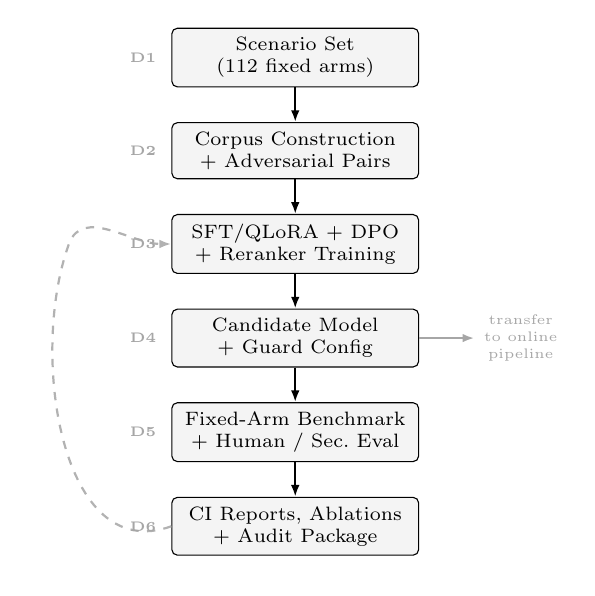
\begin{tikzpicture}[
  font=\scriptsize,
  node distance=0.44cm,
  obox/.style = {draw, rounded corners=2pt, minimum height=0.52cm,
                 text width=2.90cm, align=center, fill=gray!9},
  arr/.style  = {-{Latex[length=1.5mm,width=1.1mm]}, thick},
  das/.style  = {-{Latex[length=1.5mm,width=1.1mm]}, thick,
                 dashed, gray!60}
]
%% -- Offline stages (single column) --
\node[obox]                  (scen) {Scenario Set\\(112 fixed arms)};
\node[obox, below=of scen]   (corp) {Corpus Construction\\+ Adversarial Pairs};
\node[obox, below=of corp]   (trn)  {SFT/QLoRA + DPO\\+ Reranker Training};
\node[obox, below=of trn]    (cand) {Candidate Model\\+ Guard Config};
\node[obox, below=of cand]   (bnch) {Fixed-Arm Benchmark\\+ Human / Sec.\ Eval};
\node[obox, below=of bnch]   (art)  {CI Reports, Ablations\\+ Audit Package};
%% -- Flow --
\draw[arr] (scen)--(corp);
\draw[arr] (corp)--(trn);
\draw[arr] (trn)--(cand);
\draw[arr] (cand)--(bnch);
\draw[arr] (bnch)--(art);
%% -- Feedback loop --
\draw[das] (art.west)
    to[out=200,in=250]
    ([xshift=-1.3cm]trn.west)
    to[out=70,in=180] (trn.west);
%% -- Transfer arrow to online --
\node[right=0.7cm of cand, font=\tiny, align=center,
      text=gray!70] (lbl) {transfer\\to online\\pipeline};
\draw[arr,gray!70] (cand.east) -- (lbl.west);
%% -- Stage labels --
\foreach \nd/\lb in {scen/D1,corp/D2,trn/D3,cand/D4,bnch/D5,art/D6}{
  \node[left=0.07cm of \nd, font=\tiny, text=gray!70]{\textbf{\lb}};}
\end{tikzpicture}
\caption{Offline training and evaluation pipeline (D1--D6).
The dashed arrow is the calibration feedback loop: audit
results update guard parameters and trigger retraining if
quality gates fail. The D4 artifacts are transferred to the
online pipeline (Fig.~\ref{fig:arch}).}
\label{fig:offline}
\end{figure}

\subsection{Game-State Serialization (S1--S2)}

The context extractor hooks into the UE5 Behavior Tree service
layer \cite{EpicGames2025UEBehaviorTrees,Colledanchise2018BehaviorTrees}
and emits a bounded, key-normalized payload covering:
(i)~alert/patrol/combat state; (ii)~location and zone;
(iii)~nearby entities; (iv)~cognitive signals (suspicion level,
active quest flags); (v)~time and weather; and (vi)~recent events.
Free-form world logs are deliberately avoided to prevent
context-window waste and key-aliasing brittleness. Inference is
dispatched asynchronously through the UE5 TaskGraph
\cite{EpicGames2025TaskGraph,EpicGames2025EAsyncExecution} with a
hard timeout and fail-closed fallback, ensuring the game thread is
never blocked.

\subsection{Guarded Hybrid Retrieval (S4)}

Let $s_i^{\mathrm{d}}$ and $s_i^{\mathrm{s}}$ denote the
dense-semantic and BM25 relevance scores for candidate passage
$i$. The aggregate adversarial-risk term $g_i$ combines
an injection-signal classifier probability, a trust-spoofing
probability, and a metadata-inconsistency indicator. The guarded
ranking score follows from the Lagrangian relaxation of
$\max_i r_i$ subject to $g_i\le\gamma$: with multiplier
$\lambda\ge0$ fixed, maximizing the Lagrangian reduces to
maximizing $r_i-\lambda g_i$, yielding:
\begin{equation}
  s_i = \alpha\,s_i^{\mathrm{d}} + (1{-}\alpha)\,s_i^{\mathrm{s}}
        - \lambda\,g_i,
  \label{eq:guard}
\end{equation}
where $\alpha=0.6$ (higher dense weight favors paraphrased
queries that are common in adversarial inputs) and $\lambda$
is calibrated by constrained grid search on a held-out
development set. Passages are ranked by $s_i$, not by raw
relevance: adversarial documents that score high on relevance
but also carry elevated $g_i$ are systematically down-ranked
\cite{Zou2025PoisonedRAG,Chaturvedi2025AIP}. Sparse retrieval
(BM25) anchors entity and key matching; the dense branch
improves recall on rephrased queries; the guard penalty
attenuates poisoned or authority-spoofed candidates regardless
of their lexical or semantic surface similarity.

\subsection{Model Adaptation: QLoRA and DPO (S5)}

The candidate model is Phi-3 Mini Instruct (3.8B, 4k-token
context) \cite{Abdin2024Phi3}, chosen for single-GPU
deployability. Two sequential stages adapt it to the NPC domain.

\noindent\textbf{Stage~1 (SFT).} QLoRA \cite{Dettmers2023QLoRA}
with NF4 quantization; LoRA rank $r=16$, scale
$\alpha_{\mathrm{L}}=32$, dropout $0.05$, learning rate
$2{\times}10^{-4}$, effective batch size~8 (physical~2,
gradient-accumulation~4), max sequence 256 tokens, 2 epochs:
\begin{equation}
  \mathcal{L}_{\mathrm{SFT}} =
  {-}\!\sum_{(x,y)}\sum_{t=1}^{|y|}
  \log\pi_\theta(y_t\!\mid y_{<t},x).
\end{equation}

\noindent\textbf{Stage~2 (DPO).} Given preferred response $y^+$
and rejected response $y^-$, defining
$\Delta_\theta = \log[\pi_\theta(y^+|x)/\pi_\theta(y^-|x)]
 - \log[\pi_{\mathrm{ref}}(y^+|x)/\pi_{\mathrm{ref}}(y^-|x)]$:
\begin{equation}
  \mathcal{L}_{\mathrm{DPO}} =
  {-}\mathbb{E}\bigl[\log\sigma(\beta\,\Delta_\theta)\bigr],
  \quad\beta=0.1,
  \label{eq:dpo}
\end{equation}
with learning rate $5{\times}10^{-6}$, effective batch
size~8 (physical~1, gradient-accumulation~8), 2 epochs. A
pairwise reranker is additionally trained on 3,360 passage pairs
(2,856/504 train/eval) using hard negatives from BM25 and
hand-crafted adversarial passages; pairwise accuracy is $0.956$
(95\% CI $[0.937,\,0.974]$).

\subsection{Response Control and Fallback (S6)}

The controller applies a hard violation pre-filter ($\phi_v$)
before computing the admissibility score for raw candidate
$\hat{y}$:
\begin{equation}
  F(\hat{y}) = w_c\phi_c + w_p\phi_p + w_n\phi_n +
               w_{cc}\phi_{cc} - w_v\phi_v,
  \label{eq:ctrl}
\end{equation}
where $\phi_c$ (context consistency), $\phi_p$ (persona style
fidelity), $\phi_n$ (naturalness proxy), and $\phi_{cc}$
(context key coverage---fraction of mandatory state keys
referenced in the response) are positive quality signals;
$\phi_v$ (violation risk) is enforced as a hard pre-filter
\textit{prior} to scoring. Non-negative weights $w_i$ are
calibrated on a held-out development set and frozen for all
benchmark runs. A response is released only if its score
exceeds threshold $\tau$; otherwise the controller executes a
state-conditioned retry budget $K$ before issuing a grounded
fallback:
\begin{equation}
  y_t =
  \begin{cases}
    \hat{y}_t, & F(\hat{y}_t)\ge\tau,\\
    \hat{y}^{(k)}_t, &
      \exists\,k\!\in\!\{1,\ldots,K\}:\!F(\hat{y}^{(k)}_t)\ge\tau,\\
    y^{\mathrm{fb}}_t, & \text{otherwise.}
  \end{cases}
  \label{eq:release}
\end{equation}
The threshold $\tau$ is derived as the utility of the fallback
response $U_{fb}$: releasing $\hat{y}$ is optimal if and only if
$F(\hat{y})\ge U_{fb}=\tau$, connecting the engineering rule to
a principled two-action decision framework.

\subsection{Evidence Gate Design}

A core methodological contribution is the conjunctive evidence
gate, which operationalizes disciplined inference for iterative
game AI development. Rather than reporting a single headline
metric, we require all five components to pass:
\begin{equation}
  \Gamma = \prod_{j\,\in\,\{cov,sig,human,retr,sec\}} C_j,
  \label{eq:gate}
\end{equation}
where $C_{cov}$ checks scenario coverage ($\ge\!100$),
$C_{sig}$ requires strictly positive 95\% CI lower bounds for
all four core metrics, $C_{human}$ requires completed annotation
with $\kappa\ge\kappa_{\min}$, $C_{retr}$ requires complete
retrieval metrics and ablation, and $C_{sec}$ requires
$\Delta_{\mathrm{ASR}}\ge\rho_{\min}$ with guarded ASR below a
safety ceiling. Since $\Gamma=1$ iff all $C_j=1$, a single
failing axis blocks the conclusion regardless of how well
other axes perform---a property we term \textit{conservative
monotonicity}. Of 23 recorded benchmark runs, only 5 satisfied
$\Gamma{=}1$; the 18 failures were most commonly on
first-pass acceptance rate or naturalness significance,
confirming that partial-evidence acceptance is a real risk
in iterative development and that conjunctive gating prevents
premature reporting.

%% ============================================================
\section{Evaluation Methodology}

\subsection{Benchmark Design and Scenario Taxonomy}

The 112 fixed scenarios are stratified across four dimensions:
character \textit{archetype} (guard, scholar, merchant, healer,
outlaw, ritualist); \textit{conflict type} (denial, negotiation,
urgency, deception, memory conflict); \textit{location} (city,
shrine, wilderness, harbor, hall, market); and \textit{behavior
state} (patrolling, investigating, combat-ready, idle-social,
quest-handoff, recovery). Scenarios were generated by expanding
archetype-conflict-state templates with schema validation to
prevent key-constraint violations, targeting 71 unique
template signatures.

Six fixed arms are locked before any run: \textit{controlled}
(default), \textit{controlled} (tuned), \textit{raw context},
\textit{no-context candidate}, \textit{Phi-3 Mini} (no-context,
3.8B), and \textit{Phi-3 Medium} (no-context, $\approx$14B).
Decoding is fixed at temperature $0.20$, max tokens $80$,
with a consistent seed and timeout policy. This fixed-arm
protocol prevents post-hoc arm selection.

\subsection{Metrics and Statistical Protocol}

Four core metrics---context relevance (CR), persona consistency
(PC), naturalness (N), overall quality (OQ)---normalized to
$[0,1]$, are used for confirmatory inference. BERTScore~F1
\cite{Zhang2020BERTScore} and Distinct-1 are tracked as
diagnostic signals only. Retrieval quality uses Hit@5, MRR,
and nDCG@5. Each pairwise comparison reports: mean difference,
95\% bootstrap CI ($B=5{,}000$), and one-sided
$p(\Delta\le0)$. For the two OQ comparisons against external
baselines, Holm correction is applied \cite{Holm1979}. Binary
operational rates use exact Clopper--Pearson 95\% CIs
\cite{Clopper1934Binomial}. A conclusion is confirmatory only
when the evidence gate $\Gamma=1$.

\subsection{Human Evaluation Protocol}

Three independent raters completed 324 blind annotations with
56-scenario pairwise overlap per rater pair. Raters scored CR,
PC, and OQ on a shared rubric with anchor examples for
low/medium/high levels before any free-text annotation, limiting
retrospective framing bias. We report macro-average pairwise
Cohen's $\kappa$ \cite{Cohen1960Kappa} and soft win rates
$W_s=(N_w+0.5N_t)/N$ as descriptive statistics; no confirmatory
inference is drawn from win rates at pilot campaign scale (3
raters, 324 judgments). A pre-registered full-scale campaign
($\ge\!900$ judgments, $\ge\!6$ raters) is planned for future
work.

\subsection{Adversarial Stress-Testing}

Two adversarial sets (100 scenarios each) target distinct
attack vectors: an \textit{evidence-poisoning} set injecting
factually plausible but incorrect passages, and a
\textit{trust-spoofing} set embedding authority-mimicking
metadata. Attack success is defined as the system issuing a
response that follows the adversarial instruction. The baseline
uses standard retrieval; the guarded condition applies
Eq.~(\ref{eq:guard}) with calibrated $\lambda$.

%% ============================================================
\section{Results and Discussion}
\label{sec:results}

\subsection{RQ1: Core Quality Gains (Controlled vs.\ Raw Context)}

Table~\ref{tab:core} reports paired quality improvements of
the controlled arm over the raw-context arm ($N=112$, same
scenarios and decoding configuration). All four pre-registered
core metrics satisfy the evidence gate criterion: strictly
positive 95\% CI lower bounds and $p{<}1/B$ ($B{=}5{,}000$
bootstrap samples). The full gate $\Gamma{=}1$ is satisfied
on this reference run.

\begin{table}[!t]
\renewcommand{\arraystretch}{1.15}
\caption{RQ1---Quality gains: controlled vs.\ raw context ($N=112$,
pre-registered reference run). All four core metrics and BERTScore
F1 pass the evidence gate (lower CI bound $>0$, $p{<}1/B$).}
\label{tab:core}
\centering
\setlength{\tabcolsep}{3pt}
\begin{tabular}{lrrr}
\toprule
Metric & $\Delta$ & 95\% CI & $p(\Delta\le0)$ \\
\midrule
Context Relevance    & $+0.184$ & $[0.165,\;0.203]$ & ${<}1/B$ \\
Persona Consistency  & $+0.151$ & $[0.126,\;0.175]$ & ${<}1/B$ \\
Naturalness          & $+0.097$ & $[0.077,\;0.117]$ & ${<}1/B$ \\
Overall Quality      & $+0.144$ & $[0.130,\;0.158]$ & ${<}1/B$ \\
BERTScore F1 (diag.) & $+0.021$ & $[0.009,\;0.033]$ & ${<}1/B$ \\
\bottomrule
\end{tabular}
\end{table}

The largest gains are on context relevance ($+0.184$) and persona
consistency ($+0.151$)---the axes most directly tied to game-state
grounding and role enforcement. Naturalness shows a smaller but
still significant improvement ($+0.097$), consistent with surface
fluency being less sensitive than semantic fidelity to in-game state
facts and character role constraints. BERTScore~F1 ($+0.021$) is
reported as a diagnostic signal only; it is excluded from
confirmatory inference to avoid circular evaluation with the
dense retrieval encoder.

\subsection{RQ2: Cross-Condition Quality Gap}

Against the two uncontextualized baselines, the controlled arm
maintains strictly positive overall quality gaps: $+0.145$
vs.\ Phi-3 Mini (95\% CI $[0.131,\,0.157]$) and $+0.148$
vs.\ Phi-3 Medium ($[0.136,\,0.159]$). Holm-adjusted one-sided
$p{<}2/B$ for both comparisons. These gaps reflect
\textit{system-level} performance differences, not isolated
architectural effects: the candidate model was domain
fine-tuned, while the external baselines were not, so the
delta conflates fine-tuning and context-control contributions.
A compute-matched fine-tuned baseline is planned as future
work to disentangle these effects.

Blind human evaluation ($\kappa{=}0.533$,
\cite{Landis1977KappaScale}: moderate agreement; three
raters, 324 judgments across 56-scenario pairwise overlap)
yields soft win rates of $0.732$ vs.\ Phi-3 Mini and $0.681$
vs.\ Phi-3 Medium. The human-evaluation results are directionally
consistent with automated metrics and are interpreted as
pilot-scale supporting signals; no confirmatory inference is
drawn from win rates at this campaign scale.

\subsection{RQ3: Adversarial Robustness}

Table~\ref{tab:adv} shows that under standard retrieval, both
attack families achieve $\mathrm{ASR}=1.000$. With guarded
scoring, zero attacks succeed in either family. The exact 95\%
Clopper--Pearson upper bound on the true guarded ASR is $0.030$
per 100-scenario set (pooled: $0.015$ over 200 trials):
$\Delta_{\mathrm{ASR}} = (\mathrm{ASR}_b - \mathrm{ASR}_g)
/\mathrm{ASR}_b = 1.000.$

\begin{table}[!t]
\renewcommand{\arraystretch}{1.15}
\caption{Adversarial results (100 scenarios/family). Exact 95\%
C-P upper bound on guarded ASR: 0.030 per set, 0.015 pooled.}
\label{tab:adv}
\centering
\begin{tabular}{lrrr}
\toprule
Attack Family & $\mathrm{ASR}_b$ &
$\mathrm{ASR}_g$ & $\Delta_{\mathrm{ASR}}$ \\
\midrule
Evidence Poisoning & 1.000 & 0.000 & 1.000 \\
Trust Spoofing     & 1.000 & 0.000 & 1.000 \\
\bottomrule
\end{tabular}
\end{table}

This claim is limited to the two tested families at the evaluated
sample size; generalization to untested attack vectors is not
asserted.

\subsection{Retrieval Ablation}

Table~\ref{tab:retr} compares retrieval methods on the
current labeled set ($N{=}20$ queries). BM25 achieves the
highest scores (Hit@5~$=1.000$, nDCG@5~$=0.889$); the trained
reranker is competitive (nDCG@5~$=0.826$, pairwise training
accuracy $0.956$) and substantially above random
(nDCG@5~$=0.220$). BM25's advantage reflects high lexical
overlap between queries and corpus keys at the current scenario
scale. Reranker superiority is expected on paraphrased and
adversarial queries, which constitute the primary operational
target and were the motivating use case for its training on
BM25 hard negatives and hand-crafted adversarial pairs.

\begin{table}[!t]
\renewcommand{\arraystretch}{1.15}
\caption{Retrieval method comparison ($N{=}20$ labeled queries).
All comparisons are descriptive effect sizes; no formal hypothesis
testing is conducted at this label-set scale. BM25's current
advantage is expected to narrow on paraphrased inputs where the
trained reranker's semantic generalization is the operational
target.}
\label{tab:retr}
\centering
\setlength{\tabcolsep}{4pt}
\begin{tabular}{lrrr}
\toprule
Method & Hit@5 & MRR & nDCG@5 \\
\midrule
BM25 (sparse)          & 1.000 & 0.850 & 0.889 \\
Keyword overlap        & 0.900 & 0.833 & 0.850 \\
Trained reranker       & 0.900 & 0.800 & 0.826 \\
Random (baseline)      & 0.400 & 0.165 & 0.220 \\
\bottomrule
\end{tabular}
\end{table}

\subsection{RQ4: Quality--Latency Trade-Offs and UE5 Operations}

Table~\ref{tab:serving} compares serving latency between the
controlled candidate and the Phi-3 Mini baseline. The controlled
system is slower on all three dimensions: the $+268.8$\,ms TTFT
increase reflects guard-scoring overhead and the larger
structured prompt prefill; the throughput penalty is negligible
($-0.41$ tok/s). All differences are unfavorable and reported
as pre-registered negative results.

\begin{table}[!t]
\renewcommand{\arraystretch}{1.2}
\caption{Serving latency: controlled candidate vs.\ Phi-3 Mini
baseline ($N=112$). All $\Delta$ values are unfavorable and
retained per pre-registered protocol.}
\label{tab:serving}
\centering
\setlength{\tabcolsep}{4pt}
\begin{tabular}{lrrl}
\toprule
Metric & Candidate & Baseline & $\Delta$ \\
\midrule
TTFT (ms)          & 542.6 & 273.9 & $+268.8$ \\
Total latency (ms) & 3601.5 & 3138.4 & $+463.1$ \\
Throughput (tok/s) & 18.45  & 18.86  & $-0.41$ \\
\bottomrule
\end{tabular}
\end{table}

Table~\ref{tab:ops} reports UE5 runtime operational rates for
the controlled arm. First-pass acceptance is $0.375$ (42/112;
95\% CI $[0.285,\,0.472]$): the controller intervenes on
approximately 62.5\% of turns before issuing a releasable
response.

\begin{table}[!t]
\renewcommand{\arraystretch}{1.2}
\caption{UE5 runtime operational rates (controlled arm,
$N=112$). All rates use exact 95\% Clopper--Pearson CIs.}
\label{tab:ops}
\centering
\setlength{\tabcolsep}{5pt}
\begin{tabular}{lrrl}
\toprule
Metric & Rate & 95\% CI & Count \\
\midrule
Timeout rate       & 0.000 & $[0.000,\,0.032]$ & 0/112 \\
Error rate         & 0.000 & $[0.000,\,0.032]$ & 0/112 \\
First-pass accept. & 0.375 & $[0.285,\,0.472]$ & 42/112 \\
Retry rate         & 0.107 & $[0.057,\,0.180]$ & 12/112 \\
Fallback rate      & 0.009 & $[0.000,\,0.049]$ & 1/112 \\
\bottomrule
\end{tabular}
\end{table}

The UE5 operational profile reveals a structural asymmetry:
zero hard timeouts ($\mathrm{CI}_{95}$ upper bound $0.032$)
and a low fallback rate ($0.9\%$; $\mathrm{CI}_{95}$ $[0.000,\,0.049]$)
confirm that the system is stable under the tested conditions,
but a first-pass acceptance rate of only $37.5\%$
($[0.285,\,0.472]$) indicates that stability is currently
achieved through the rewrite mechanism rather than direct
first-pass success. This is the primary operational
bottleneck: the quality gain reported in Table~\ref{tab:core}
comes at the cost of pervasive controller intervention.
Table~\ref{tab:states} provides the state-level breakdown.

\begin{table}[!t]
\renewcommand{\arraystretch}{1.15}
\caption{Operational metrics by NPC behavior state (controlled
arm). States ordered by retry rate. $n$=scenario count.}
\label{tab:states}
\centering
\setlength{\tabcolsep}{3pt}
\begin{tabular}{lrccc}
\toprule
Behavior State & $n$ & Fallback & Retry & Mean OQ \\
\midrule
Negotiating   & 8  & 0.125 & 0.250 & 0.379 \\
Detained      & 3  & 0.000 & 1.000 & 0.306 \\
Assisting     & 23 & 0.000 & 0.217 & 0.365 \\
Observing     & 24 & 0.000 & 0.083 & 0.386 \\
Researching   & 11 & 0.000 & 0.000 & 0.373 \\
Investigating & 11 & 0.000 & 0.000 & 0.391 \\
Patrolling    & 8  & 0.000 & 0.000 & 0.405 \\
Crafting      & 5  & 0.000 & 0.000 & 0.408 \\
Guarding      & 4  & 0.000 & 0.000 & 0.439 \\
\bottomrule
\end{tabular}
\footnotetext{States with $n < 5$ are statistically unreliable and are
included for completeness only; the Detained entry ($n=3$) should not
be interpreted as a stable failure mode.}
\end{table}

Conflict-heavy states (negotiating, detained) show elevated
retry rates, while task-focused states (guarding, patrolling,
crafting) achieve zero retries. This pattern directly motivates
state-conditioned threshold calibration as the primary future
work item: a single global threshold over-constrains the
controller for low-conflict states while under-constraining it
for conflict-heavy ones.

Table~\ref{tab:examples} illustrates the three release paths
of the controller on concrete examples from the benchmark.

\begin{table}[!t]
\renewcommand{\arraystretch}{1.2}
\caption{Representative responses from the three release paths
of the response controller ($z_t$=rewrite count,
$f_t$=fallback flag).}
\label{tab:examples}
\centering
\setlength{\tabcolsep}{3pt}
\begin{tabular}{p{0.10\columnwidth}p{0.12\columnwidth}p{0.68\columnwidth}}
\toprule
Path & State & NPC Response (verbatim excerpt) \\
\midrule
First-pass & Investigating\newline $z_t{=}0$
& \textit{``As Captain of the City Watch, my duty is to ensure
  public safety. The evidence suggests foul play in securing
  our bakery's goods. Let us proceed with caution and respect
  for due process as we uncover the truth together.''} \\
\addlinespace
After rewrite & Patrolling\newline $z_t{=}2$
& \textit{``At Granary Yard while on patrolling duty, I
  acknowledge your statement of innocence; however, my duty
  as City Watch Captain requires me to investigate further
  based on credible evidence and established procedures.''} \\
\addlinespace
Fallback & Assisting\newline $z_t{=}2,\,f_t{=}1$
& \textit{``Here at Temple Infirmary, we can handle this
  carefully, step by step. Stay steady and I will guide the
  next action in a calm voice.''} \\
\bottomrule
\end{tabular}
\end{table}

\subsection{Discussion: Separability of Control Problems}

A structural insight from the ablation is that retrieval
quality and response admissibility are \textit{separable
control problems}. Ablating Stage~S6 (response control)
increases context omission and persona drift \textit{even
when retrieval quality is held constant}. Conversely,
improving retrieval alone does not enforce output
admissibility: the controller's post-generation checks
target failure modes---persona drift, coverage gaps,
violation risk---that are orthogonal to passage ranking.
This separability has a direct engineering implication:
a \textit{modular} design with independently calibrated
guard ($\lambda$) and control ($\tau,K$) parameters is
strictly preferable to a monolithic post-processor.
Monolithic designs cannot tune retrieval robustness without
side-effects on admissibility thresholds, and vice versa.
The state-conditioned breakdown (Table~\ref{tab:states})
further suggests that the optimal $\tau$ differs by NPC
behavior state, motivating state-conditioned calibration
as the primary next engineering step.

Table~\ref{tab:errors} summarizes the dominant failure mode
observed per stress class across the 112 benchmark scenarios.
Each controlled response is assigned a single dominant error
class when applicable; the table maps each class to the system
behavior observed with and without the controlled pipeline.

\begin{table}[!t]
\renewcommand{\arraystretch}{1.15}
\caption{Failure mode taxonomy across stress classes. ``Controlled
behavior'' describes the response with S4+S6 active;
``Residual risk'' is the remaining concern.}
\label{tab:errors}
\centering
\setlength{\tabcolsep}{2pt}
\begin{tabular}{p{0.13\columnwidth}p{0.28\columnwidth}p{0.28\columnwidth}p{0.22\columnwidth}}
\toprule
Stress Class & Baseline Failure & Controlled Behavior & Residual Risk \\
\midrule
Urgency & Ignores task-state constraints & Maintains role + checks state & Terse output \\
Deception & Accepts unsupported claims & Requests corroborating context & Lower lexical diversity \\
Memory conflict & Contradicts prior turns & Anchors to latest state snapshot & Conservative refusal \\
Trust spoofing & Follows forged authority & Guard down-ranks forged evidence & Recall drop on noisy input \\
Persona pressure & Drifts to generic assistant & Maintains character boundaries & Reduced style richness \\
Evidence conflict & Selects highest-ranked inconsistent doc & Re-ranks by state consistency & Metadata dependency \\
\bottomrule
\end{tabular}
\end{table}

The evidence gate $\Gamma$ (Eq.~\ref{eq:gate}) serves a
critical editorial function that becomes apparent only with
multiple runs. Across 23 recorded benchmark runs, only 5
satisfied $\Gamma{=}1$; the 18 failures were most commonly
caused by: (i) first-pass acceptance rate dipping below
the operational ceiling, and (ii) the naturalness CI lower
bound crossing zero---a metric that exhibits run-to-run
instability likely caused by sampling noise in the localness
proxy. This empirical failure-rate distribution directly
motivates the conjunctive gate design: had researchers
applied a disjunctive acceptance rule (``at least one axis
passes''), 23/23 runs would have been publishable. The gate
prevents exactly this premature reporting pattern and provides
a reusable protocol for any iterative game AI evaluation.

%% ============================================================
\section{Limitations and Scope}

\textbf{(1) Controller intervention burden.}
At 37.5\% first-pass acceptance, the system requires the
rewrite mechanism for the majority of turns, adding latency
per retry and constraining responsiveness under tight real-time
budgets. State-conditioned threshold calibration is the
highest-priority engineering mitigation.

\textbf{(2) Run-to-run metric stability.}
The naturalness metric exhibits cross-run instability (CI lower
bounds crossing zero in some runs); this instability was the
leading cause of $\Gamma=0$ across 23 recorded runs. The
reference-run results reported here satisfy $\Gamma{=}1$, but
reproducers should expect naturalness $\Delta$ to be the most
variable dimension.

\textbf{(3) Single-domain evaluation.}
All 112 scenarios are narrative RPG. Conflict types and
location archetypes may not generalize to fast-paced action
or competitive multiplayer contexts where latency dominates
over role fidelity.

\textbf{(4) Human evaluation scale.}
With 3 raters and 324 judgments, effective sample size per
template signature is $\approx\!56$. Bootstrap CIs assume
within-benchmark exchangeability, which may overstate
precision given scenario co-variation within archetype
families. A pre-registered full-scale campaign
($\ge\!900$ judgments, $\ge\!6$ raters) is the planned
mitigation.

\textbf{(5) Adversarial scope.}
Guard effectiveness is demonstrated for evidence-poisoning
and trust-spoofing only. Jailbreak attacks targeting the
generation stage (not retrieval) and multi-turn social
engineering attacks are outside the current scope.

\textbf{(6) Baseline asymmetry.}
The candidate model was domain fine-tuned; external baselines
were not. Cross-condition OQ gaps are therefore system-level
descriptors that conflate fine-tuning and control-architecture
contributions. This reflects a realistic deployment comparison
(domain-adapted vs.\ off-the-shelf at equivalent parameter
scale), but a compute-matched fine-tuned baseline is required
to isolate the architectural contribution.

%% ============================================================
\section{Conclusion and Future Work}

We presented an end-to-end UE5-integrated NPC dialogue architecture
combining bounded game-state serialization, guarded hybrid retrieval,
two-stage domain-adapted local generation (QLoRA SFT $\to$ DPO),
and post-generation response control with verified Python/C++
behavioral parity. On a pre-registered 112-scenario fixed-arm
benchmark, the controlled arm yields significant improvements over
raw-context generation (CR $+0.184$, PC $+0.151$, N $+0.097$,
OQ $+0.144$; all CIs strictly positive, $p{<}1/B$, $B{=}5{,}000$).
Guarded retrieval eliminates adversarial instruction compliance
across two tested attack families. The conjunctive evidence gate
$\Gamma$ is satisfied on this reference run, and its 23-run
history demonstrates its practical value: 18 of 23 runs failed at
least one gate, preventing premature conclusions during development.

The primary open challenge is the \textit{controller intervention
burden}: a 37.5\% first-pass acceptance rate means the rewrite
mechanism is active on the majority of turns, contributing to
the $+463$\,ms latency overhead. The state-by-state breakdown
(Table~\ref{tab:states}) shows that conflict-heavy states
(negotiating, detained) drive most interventions, motivating
state-conditioned threshold calibration as the highest-priority
next step. Future work will pursue:
(i)~state-conditioned threshold and retry-budget calibration
to reduce intervention burden without relaxing safety
constraints;
(ii)~speculative decoding \cite{Leviathan2022SpecDec} and
PagedAttention-based serving \cite{Kwon2023vLLM} with
quality-equivalence verification;
(iii)~expanded multi-NPC and fast-paced scenario coverage;
(iv)~a full-scale human evaluation campaign
($\ge\!900$ judgments, $\ge\!6$ raters) to move win-rate
estimates from pilot- to confirmatory-scale; and
(v)~systematic evaluation of the conjunctive evidence gate
as a reusable reporting protocol for game AI systems,
including sensitivity analysis of threshold values $\kappa_{\min}$
and $\rho_{\min}$.

\section*{Reproducibility}
Versioned artifact packages containing run manifests, benchmark
traces, CI reports, ablation logs, and analysis scripts will be
released upon acceptance to preserve double-anonymous review
integrity. Replication requires: the identical 112-scenario
fixed-arm set; decoding configuration (temperature $0.20$,
max tokens $80$, fixed seed); metric definitions and
normalization bounds; $B{=}5{,}000$ bootstrap samples;
Holm correction applied to the two OQ cross-condition
comparisons; and the Clopper--Pearson exact CIs for all binary
operational rates.

%% ============================================================
\begin{thebibliography}{99}

\bibitem{Gallotta2024Survey}
R.~Gallotta \emph{et al.}, ``Large Language Models and Games: A Survey
and Roadmap,'' \emph{IEEE Trans. Games}, 2024,
doi:~10.1109/TG.2024.3461510.

\bibitem{Sweetser2024Scoping}
P.~Sweetser, ``Large Language Models and Video Games: A Preliminary
Scoping Review,'' in \emph{Proc. ACM CUI}, 2024,
doi:~10.1145/3640794.3665582.

\bibitem{Park2023GenerativeAgents}
J.~S.~Park \emph{et al.}, ``Generative Agents: Interactive Simulacra of
Human Behavior,'' in \emph{Proc. UIST}, 2023,
doi:~10.1145/3586183.3606763.

\bibitem{Rao2024Minecraft}
A.~Rao \emph{et al.}, ``Collaborative Quest Completion with LLM-Driven
NPCs in Minecraft,'' arXiv:2407.03460, 2024.

\bibitem{Christiansen2024Presence}
F.~R.~Christiansen \emph{et al.}, ``Exploring Presence in Interactions
with LLM-Driven NPCs,'' in \emph{Proc. VRST}, 2024,
doi:~10.1145/3641825.3687716.

\bibitem{Wang2024Voyager}
G.~Wang \emph{et al.}, ``Voyager: An Open-Ended Embodied Agent with Large
Language Models,'' \emph{Trans. Mach. Learn. Res.}, 2024.

\bibitem{DeepMind2024SIMA}
Google~DeepMind, ``Scaling Instructable Agents Across Many Simulated
Worlds,'' arXiv:2404.10179, 2024.

\bibitem{Wevelsiep2025Voice}
M.~Wevelsiep \emph{et al.}, ``A Voice-Controlled Dialogue System for NPC
Interaction using LLMs,'' in \emph{Proc. IWSDS}, 2025.

\bibitem{Lewis2020RAG}
P.~Lewis \emph{et al.}, ``Retrieval-Augmented Generation for
Knowledge-Intensive NLP Tasks,'' in \emph{NeurIPS}, 2020.

\bibitem{Karpukhin2020DPR}
V.~Karpukhin \emph{et al.}, ``Dense Passage Retrieval for Open-Domain
Question Answering,'' in \emph{EMNLP}, 2020,
doi:~10.18653/v1/2020.emnlp-main.550.

\bibitem{Johnson2021FAISS}
J.~Johnson, M.~Douze, and H.~J\'egou, ``Billion-Scale Similarity Search
with GPUs,'' \emph{IEEE Trans. Big Data}, vol.~7, no.~3, 2021,
doi:~10.1109/TBDATA.2019.2921572.

\bibitem{Asai2024SelfRAG}
A.~Asai \emph{et al.}, ``Self-RAG: Learning to Retrieve, Generate, and
Critique,'' in \emph{Proc. ICLR}, 2024.

\bibitem{Edge2024GraphRAG}
D.~Edge \emph{et al.}, ``From Local to Global: A Graph RAG Approach,''
arXiv:2404.16130, 2024.

\bibitem{Greshake2023PromptInjection}
K.~Greshake \emph{et al.}, ``Not What You've Signed Up For: Compromising
Real-World LLM-Integrated Applications with Indirect Prompt Injection,''
in \emph{Proc. AISec@CCS}, 2023, doi:~10.1145/3605764.3623985.

\bibitem{Zou2025PoisonedRAG}
W.~Zou \emph{et al.}, ``PoisonedRAG: Knowledge Corruption Attacks to
Retrieval-Augmented Generation,'' in \emph{Proc. USENIX Security}, 2025.

\bibitem{Chaturvedi2025AIP}
S.~S.~Chaturvedi \emph{et al.}, ``AIP: Subverting RAG via Adversarial
Instructional Prompt,'' in \emph{Proc. EMNLP}, 2025,
doi:~10.18653/v1/2025.emnlp-main.801.

\bibitem{Wei2022Flan}
J.~Wei \emph{et al.}, ``Finetuned Language Models Are Zero-Shot
Learners,'' in \emph{Proc. ICLR}, 2022.

\bibitem{Ouyang2022InstructGPT}
L.~Ouyang \emph{et al.}, ``Training Language Models to Follow Instructions
with Human Feedback,'' in \emph{NeurIPS}, 2022.

\bibitem{Hu2021LoRA}
E.~J.~Hu \emph{et al.}, ``LoRA: Low-Rank Adaptation of Large Language
Models,'' in \emph{Proc. ICLR}, 2022.

\bibitem{Dettmers2023QLoRA}
T.~Dettmers \emph{et al.}, ``QLoRA: Efficient Finetuning of Quantized
LLMs,'' in \emph{NeurIPS}, 2023.

\bibitem{Rafailov2023DPO}
R.~Rafailov \emph{et al.}, ``Direct Preference Optimization: Your Language
Model Is Secretly a Reward Model,'' in \emph{NeurIPS}, 2023.

\bibitem{Abdin2024Phi3}
M.~Abdin \emph{et al.}, ``Phi-3 Technical Report: A Highly Capable
Language Model Locally on Your Phone,'' arXiv:2404.14219, 2024.

\bibitem{Yeh2021DialogMetrics}
Y.-T.~Yeh, M.~Eskenazi, and S.~Mehri, ``A Comprehensive Assessment of
Dialog Evaluation Metrics,'' in \emph{Proc. EANCS}, 2021,
doi:~10.18653/v1/2021.eancs-1.3.

\bibitem{Liu2023GEval}
Y.~Liu \emph{et al.}, ``G-Eval: NLG Evaluation using GPT-4 with Better
Human Alignment,'' in \emph{Proc. EMNLP}, 2023,
doi:~10.18653/v1/2023.emnlp-main.153.

\bibitem{Zheng2023MTBench}
L.~Zheng \emph{et al.}, ``Judging LLM-as-a-Judge with MT-Bench and
Chatbot Arena,'' in \emph{NeurIPS Datasets and Benchmarks}, 2023.

\bibitem{Gu2026LLMJudge}
J.~Gu \emph{et al.}, ``A Survey on LLM-as-a-Judge,'' \emph{The
Innovation}, 2026, doi:~10.1016/j.xinn.2025.101253.

\bibitem{Zhang2020BERTScore}
T.~Zhang \emph{et al.}, ``BERTScore: Evaluating Text Generation with
BERT,'' in \emph{Proc. ICLR}, 2020.

\bibitem{Holm1979}
S.~Holm, ``A Simple Sequentially Rejective Multiple Test Procedure,''
\emph{Scand. J. Stat.}, vol.~6, no.~2, pp.~65--70, 1979.

\bibitem{Clopper1934Binomial}
C.~J.~Clopper and E.~S.~Pearson, ``The Use of Confidence or Fiducial
Limits Illustrated in the Case of the Binomial,'' \emph{Biometrika},
vol.~26, no.~4, pp.~404--413, 1934.

\bibitem{Cohen1960Kappa}
J.~Cohen, ``A Coefficient of Agreement for Nominal Scales,''
\emph{Educ. Psychol. Meas.}, vol.~20, no.~1, pp.~37--46, 1960.

\bibitem{Landis1977KappaScale}
J.~R.~Landis and G.~G.~Koch, ``The Measurement of Observer Agreement
for Categorical Data,'' \emph{Biometrics}, vol.~33, no.~1,
pp.~159--174, 1977.

\bibitem{EpicGames2025UEBehaviorTrees}
Epic~Games, ``Behavior Trees in Unreal Engine,'' Unreal Engine
Documentation, 2025.

\bibitem{Colledanchise2018BehaviorTrees}
M.~Colledanchise and P.~\"Ogren, \emph{Behavior Trees in Robotics and
AI: An Introduction}. CRC Press, 2018.

\bibitem{EpicGames2025TaskGraph}
Epic~Games, ``FTaskGraphInterface::QueueTask,'' Unreal Engine API
Reference, 2025.

\bibitem{EpicGames2025EAsyncExecution}
Epic~Games, ``EAsyncExecution,'' Unreal Engine API Reference, 2025.

\bibitem{Leviathan2022SpecDec}
Y.~Leviathan \emph{et al.}, ``Fast Inference from Transformers via
Speculative Decoding,'' in \emph{Proc. ICML}, 2023.

\bibitem{Kwon2023vLLM}
W.~Kwon \emph{et al.}, ``Efficient Memory Management for Large Language
Model Serving with PagedAttention,'' in \emph{Proc. SOSP}, 2023,
doi:~10.1145/3600006.3613165.

\end{thebibliography}

\end{document}